\begin{frame}
\centering
\begin{tabular}{|l|l|}
\hline
       & Content \\
\hline\hline
Week 1 & Basic expressions  \\
\hline
Week 2 & procedure declarations \\
\hline
Week 3 & if-statement \\
\hline
Week 4 & while-statement \\
\hline
Week 5 & for-statement \\
\hline
\ldots & \\
\end{tabular}
\end{frame}


%%%%% SICP
\begin{frame}
\centering
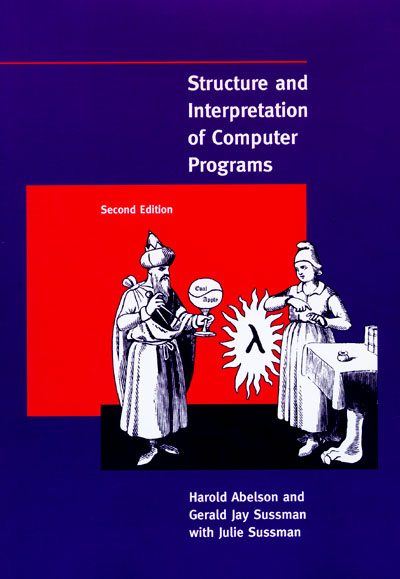
\includegraphics{sicp.jpg}
\end{frame}


\begin{frame}[fragile]
\begin{schemecode}
(define (factorial n)
  (if (<= n 1)
      1
      (* n (factorial (- n 1)))))
\end{schemecode}
\end{frame}


\iffalse
\begin{frame}[fragile]
\begin{schemecode}
(define (map proc items)
  (if (null? items)
      nil
      (cons (proc (car items))
            (map proc (cdr items)))))
\end{schemecode}
\end{frame}


\begin{frame}[fragile]
\begin{schemecode}
(define (abs x)
  (cond ((> x 0) x)
        ((= x 0) x)
        ((< x 0) (- x))))
\end{schemecode}
\end{frame}
\fi


\begin{frame}[fragile]
Evaluation by substitution

\begin{schemecode}
(define (sum-of-squares x y)
  (+ (sqr x) (sqr y)))
\end{schemecode}

\nl
\hrule
\pnl

\begin{schemecode}
     (sum-of-squares 3 4)
\end{schemecode}
\pause
\begin{schemecode}
=>   (+ (sqr 3) (sqr 4))
\end{schemecode}
\pause
\begin{schemecode}
=>   (+ (* 3 3) (sqr 4))
\end{schemecode}
\pause
\begin{schemecode}
=>   (+ 9 (sqr 4))
\end{schemecode}
\pause
\begin{schemecode}
=>   (+ 9 (* 4 4))
\end{schemecode}
\pause
\begin{schemecode}
=>   (+ 9 16)
\end{schemecode}
\pause
\begin{schemecode}
=>   25
\end{schemecode}
\end{frame}


\begin{frame}
\centering

\includegraphics[scale=0.8]{sicp-factorial.png}
\end{frame}


\begin{frame}

\begin{center}
{\bf Incredible breadth of content}
\end{center}
%\begin{center} recursion \end{center}
\begin{center} complexity analysis \end{center}
\begin{center} symbolic computation with quotation \end{center}
%\begin{center} meta-linguistic abstraction \end{center}
\begin{center} interpreters \end{center}
\begin{center} object-oriented programming \end{center}
\begin{center} logic programming \end{center}
\begin{center} many other concepts \end{center}
\end{frame}

